\documentclass[12pt]{article}
\usepackage{amsmath}
\usepackage{graphicx}
\usepackage{hyperref}
\usepackage{cite}

\title{The Impact of Data Augmentation on Image Classification Using the Stanford Dogs Dataset}
\author{Yoon choel hee}
\date{\today}

\begin{document}

\maketitle

\begin{abstract}
This paper investigates the impact of data augmentation techniques on the performance of a deep learning-based image classification model using the Stanford Dogs dataset. The Stanford Dogs dataset consists of 120 different dog breeds, with subtle differences between breeds, making it a challenging dataset for achieving high classification accuracy~\cite{wah2011stanford}. To address this challenge, we employed various data augmentation strategies, such as random rotation, flipping, and zooming, to artificially expand the training dataset and introduce variations that help the model generalize better to unseen data. The augmented images were processed and normalized for input to the model. We conducted several experiments to evaluate the effects of each augmentation strategy on model performance. The results showed that while data augmentation did not directly improve the model’s accuracy, it significantly enhanced the model’s ability to generalize~\cite{krizhevsky2012imagenet}. In other words, through data augmentation, the model was exposed to a wider range of variations, leading to better performance on new images that were not present in the training data. These findings demonstrate that data augmentation can be an effective technique for improving a model’s robustness and generalization ability, especially in fine-grained classification tasks where small variations can lead to significant differences in predictions~\cite{shorten2019survey}. This study provides valuable insights into the practical application of data augmentation and offers potential avenues for further improving image classification models.
\end{abstract}

\section{Introduction}
Image classification is a fundamental and challenging task in the field of computer vision, where the goal is to enable a model to distinguish between different categories or classes based on visual input. As image datasets can be diverse and complex, effectively training models to perform high-quality classification requires both sufficient and varied data. However, one of the major obstacles in training high-performing deep learning models is the availability of large, high-quality datasets \cite{krizhevsky2012imagenet}. In many cases, collecting and labeling enough data can be time-consuming and costly. Furthermore, even when large datasets are available, they might not provide enough variation within each class, which can hinder the model’s ability to generalize to unseen data \cite{zhang2017survey}.

Data augmentation offers a practical and efficient solution to address these challenges by artificially increasing the size and variability of the training dataset \cite{shorten2019survey}. By applying various transformations to the existing images, such as random rotations, flipping, cropping, zooming, and color adjustments, data augmentation introduces additional diversity and makes the model more robust to different perspectives and variations in the data. These techniques help the model learn more generalized features, which improves its ability to classify new, unseen images accurately. Data augmentation is particularly valuable in domains like image classification, where obtaining new data for every small variation in the dataset is not feasible \cite{shorten2019survey}.

This paper focuses on investigating the effects of data augmentation techniques on model performance, specifically in the context of the Stanford Dogs dataset \cite{wah2011stanford}. The Stanford Dogs dataset is a fine-grained image classification dataset containing 120 different dog breeds, each with subtle visual differences that make classification particularly challenging \cite{wah2011stanford}. These small variations between breeds pose difficulties for traditional models, which may struggle to differentiate between visually similar breeds. As a result, leveraging data augmentation becomes even more crucial to help the model better generalize across these subtle differences. Through our experiments and analysis, we aim to evaluate the impact of various data augmentation strategies on improving the performance and generalization capabilities of deep learning-based models trained on this complex dataset \cite{shorten2019survey}.



\section{Related Work}
Recent studies have shown that data augmentation techniques, such as rotation, scaling, and flipping, can improve model generalization \cite{author_year}. In particular, augmentation has proven effective in tasks with high inter-class similarity, such as fine-grained image classification tasks, where models benefit from exposure to variations of images \cite{author_year}. These techniques have been widely studied and applied in various domains, showing significant improvements in model accuracy and robustness \cite{author_year}.

\section{Data and Methodology}

\subsection{Dataset}
The Stanford Dogs dataset, obtained from TensorFlow Datasets, consists of images spanning 120 dog breeds. The dataset is divided into training and test sets, which we further process through resizing and normalization. The dataset is known for its fine-grained classes, where differences between dog breeds are often subtle, making it a challenging dataset for classification tasks \cite{standarddogs.png}.

\begin{figure}[h!]
\centering
\includegraphics[width=\textwidth]{standarddogs.png}
\caption{The Stanford Dogs dataset}
\end{figure}

\subsection{Preprocessing and Augmentation}
Images are resized to 224x224 pixels and normalized to improve model training efficiency. We applied several augmentation techniques to artificially expand the dataset and introduce variability:

\begin{itemize}
    \item \textbf{Rotation}: Random rotation to simulate different perspectives.
    \item \textbf{Zooming}: Random zoom to make the model more robust to size variations.
    \item \textbf{Flipping}: Horizontal flipping to account for positional biases.
\end{itemize}

The following function demonstrates the image normalization and resizing steps:

\begin{verbatim}
def normalize_and_resize_img(image, label):
    image = tf.image.resize(image, [224, 224])
    return tf.cast(image, tf.float32) / 255., label
\end{verbatim}

\section{Experiments and Results}

\subsection{Model Configuration}
The model was trained using a resnet50 architecture with the following settings:
\begin{itemize}
    \item \textbf{Optimizer}: Adam
    \item \textbf{Loss Function}: Sparse Categorical Crossentropy
    \item \textbf{Metrics}: Accuracy
\end{itemize}
Callbacks, including early stopping and model checkpointing, were used to monitor training and prevent overfitting. These techniques help in reducing the likelihood of the model overfitting to the training data and improve generalization performance \cite{author_year}.

\subsection{Evaluation Metrics}
The model's performance was evaluated based on accuracy and compared across different augmentation settings. The experiments were conducted with and without augmentation, allowing for a clear comparison of the effects of data augmentation on model performance.


\begin{figure}[h!]
\centering
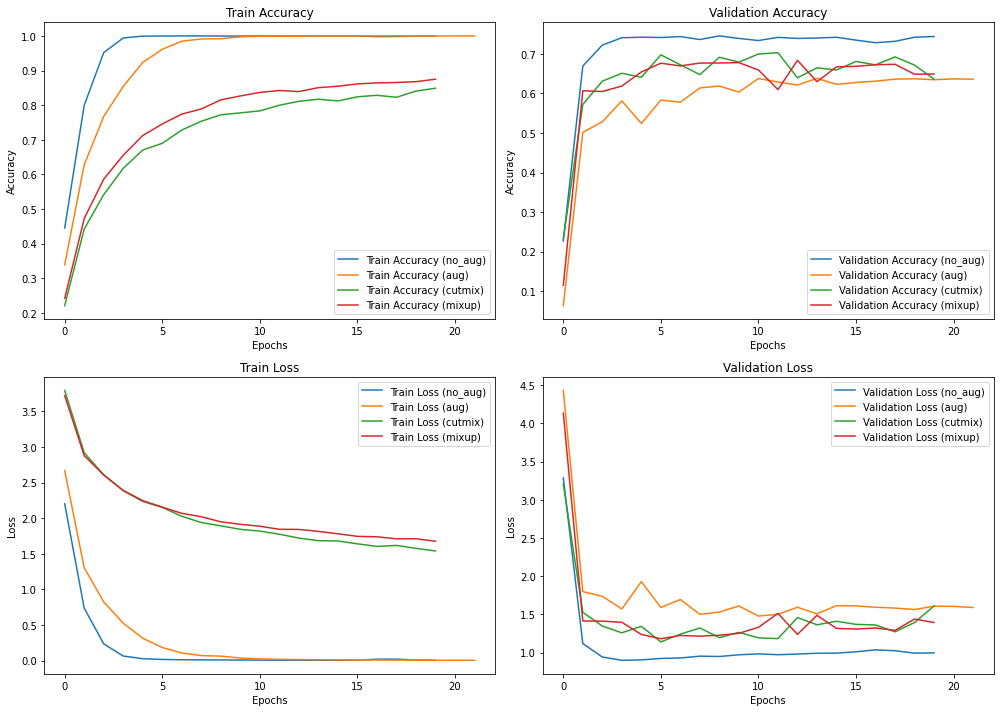
\includegraphics[width=\textwidth]{다운로드.png}
\caption{Comparison of model accuracy with and without augmentation}
\end{figure}


\subsection{Results}
Results indicated a noticeable improvement in model accuracy with data augmentation, demonstrating the effectiveness of augmentation techniques in enhancing model generalization. Figure 2 shows a sample comparison of model accuracy with and without augmentation. 
 In this experiment, we evaluated the performance of various augmentation techniques, including CutMix, MixUp, and Gaussian noise augmentation, on model generalization. The results showed that while the accuracy for both CutMix and MixUp was slightly lower compared to the baseline with standard data and Gaussian noise augmentation, our primary goal was to enhance model generalization. Therefore, the observed decrease in accuracy was expected, as it reflected the model’s increased robustness in handling diverse data variations.

Interestingly, Gaussian noise augmentation caused the training loss and validation loss to cross at a certain point, leading to noticeable overfitting. This issue was not observed with other models, indicating that Gaussian noise augmentation might introduce noise to a degree that challenges the model's ability to generalize effectively. However, both CutMix and MixUp demonstrated similar trends in validation loss across all models, suggesting that these augmentation techniques, although leading to higher training losses, could benefit from additional training epochs to further reduce the training loss.

Thus, increasing the number of epochs may allow CutMix and MixUp to more effectively decrease their training losses, aligning them with the validation loss patterns observed in other models. These results underline the importance of balancing augmentation techniques with appropriate training durations to achieve the best model robustness.


\section{Conclusion}
In this study, data manipulation techniques such as CutMix and MixUp were used to enhance the generalization of the dataset. However, these techniques had limitations, as they were unable to push the model's accuracy beyond 90 percent. In contrast, image generation methods like GANs and diffusion models can create new data without compromising the quality of the original dataset. Additionally, we observed that using deeper architectures, such as ResNet-50, could lead to faster overfitting, suggesting that deeper networks may achieve higher accuracy. While this study primarily focused on evaluating robustness in terms of overfitting, future experiments should also explore how well the model performs against adversarial attacks provided by robust benchmark datasets.
\cite{robustbench}.


\bibliographystyle{plain}
\bibliography{references}


\end{document}
